% Clinical TabReD Lite -- IEEE conference-style report.
% All numeric tables come from tables/*.tex and every number in the text is a \kn{...}
% macro from tables/numbers.tex; both are generated from ../results by
%   python -m clinical_tabred.run --stage report
% Passages marked with \STUDENT{...} must be written by the students in their own words.
\documentclass[conference]{IEEEtran}
\usepackage[T1]{fontenc}  % gives Times (IEEE body font) with pdfLaTeX and tectonic
\usepackage{graphicx}
\usepackage{booktabs}
\usepackage{amsmath,amssymb}
\usepackage{algorithm}
\usepackage{algpseudocode}
\usepackage{xcolor}
\usepackage{url}
\usepackage{cite}
\graphicspath{{../figures/}}
% Generated from the results folder by report_tables.py. Do not edit by hand.
\makeatletter
\newcommand{\kn}[1]{\@nameuse{kn@#1}}
\@namedef{kn@best_model}{XGBoost}
\@namedef{kn@seed}{42}
\@namedef{kn@n_2011}{5{,}202}
\@namedef{kn@prevalence_2011}{13.0\%}
\@namedef{kn@weighted_prevalence_2011}{9.4\%}
\@namedef{kn@n_2013}{5{,}416}
\@namedef{kn@prevalence_2013}{13.1\%}
\@namedef{kn@weighted_prevalence_2013}{10.4\%}
\@namedef{kn@n_2015}{5{,}346}
\@namedef{kn@prevalence_2015}{15.1\%}
\@namedef{kn@weighted_prevalence_2015}{11.3\%}
\@namedef{kn@n_total}{15{,}964}
\@namedef{kn@best_temporal_roc_auc}{0.791}
\@namedef{kn@best_temporal_roc_auc_low}{0.775}
\@namedef{kn@best_temporal_roc_auc_high}{0.807}
\@namedef{kn@best_temporal_pr_auc}{0.368}
\@namedef{kn@best_temporal_pr_auc_low}{0.339}
\@namedef{kn@best_temporal_pr_auc_high}{0.402}
\@namedef{kn@best_temporal_f1}{0.444}
\@namedef{kn@best_temporal_recall}{0.656}
\@namedef{kn@best_temporal_precision}{0.336}
\@namedef{kn@best_temporal_accuracy}{0.752}
\@namedef{kn@best_temporal_threshold}{0.60}
\@namedef{kn@a2_gap_roc_auc_diff}{+0.036}
\@namedef{kn@a2_gap_roc_auc_diff_low}{-0.001}
\@namedef{kn@a2_gap_roc_auc_diff_high}{+0.070}
\@namedef{kn@random_minus_temporal_roc_auc_diff}{-0.004}
\@namedef{kn@random_minus_temporal_roc_auc_diff_low}{-0.033}
\@namedef{kn@random_minus_temporal_roc_auc_diff_high}{+0.023}
\@namedef{kn@random_roc_auc_mean}{0.804}
\@namedef{kn@random_n_seeds}{5}
\@namedef{kn@random_roc_auc_std}{0.015}
\@namedef{kn@cv_temporal_roc_auc_mean}{0.804}
\@namedef{kn@cv_temporal_roc_auc_std}{0.007}
\@namedef{kn@domain_auc_2015}{0.582}
\@namedef{kn@max_ks_2015}{0.057}
\@namedef{kn@ablation_demographic_delta_roc_auc}{-0.086}
\@namedef{kn@ablation_anthropometric_delta_roc_auc}{-0.043}
\@namedef{kn@mlp_best_epoch}{22}
\makeatother


\newcommand{\STUDENT}[1]{\par\smallskip\noindent\fcolorbox{red!70!black}{yellow!12}{%
  \parbox{\dimexpr\linewidth-2\fboxsep-2\fboxrule}{\small\textbf{STUDENT TO WRITE:} #1}}\par\smallskip}

\begin{document}

\title{Evaluating Tabular Machine Learning Models under Temporal Distribution Shift in Healthcare Data\\
\large Clinical TabReD Lite (CSCI 447 Project P034)}

\author{\IEEEauthorblockN{STUDENT\_NAME\_1 (STUDENT\_ID\_1) \quad STUDENT\_NAME\_2 (STUDENT\_ID\_2)}
\IEEEauthorblockA{Department of Computer Science, SCAI, Nazarbayev University\\
Course: CSCI 447 Machine Learning: Theory and Practice, Fall 2026\\
Instructor: Dr. Hari Mohan Rai}}

\maketitle

\begin{abstract}
Models trained on past data are applied to people seen later, so random train/test splits may
misjudge their performance. Inspired by the TabReD benchmark~\cite{rubachev2024tabred}, we compare
logistic regression, random forest, XGBoost, LightGBM and a multilayer perceptron on three NHANES
survey cycles (2011--2016)~\cite{nhanes}, predicting self-reported diagnosed diabetes in
\kn{n_total} adults from nine demographic, socioeconomic and body-measurement features. Under a
chronological protocol (train 2011--2012, validate 2013--2014, test 2015--2016) the
validation-selected model (\kn{best_model}) reaches ROC-AUC \kn{best_temporal_roc_auc}
(95\% CI \kn{best_temporal_roc_auc_low}--\kn{best_temporal_roc_auc_high}) and PR-AUC
\kn{best_temporal_pr_auc}. The difference between a random-split test and the chronological test
is \kn{random_minus_temporal_roc_auc_diff} ROC-AUC (95\% CI \kn{random_minus_temporal_roc_auc_diff_low}
to \kn{random_minus_temporal_roc_auc_diff_high}), and the same fitted model scores
\kn{a2_gap_roc_auc_diff} higher on an in-period holdout than on the future cycle (95\% CI
\kn{a2_gap_roc_auc_diff_low} to \kn{a2_gap_roc_auc_diff_high}). Covariate shift is mild
(largest KS statistic \kn{max_ks_2015}; domain-classifier ROC-AUC \kn{domain_auc_2015}) while
prevalence rises from \kn{prevalence_2011} to \kn{prevalence_2015}.
\end{abstract}

\begin{IEEEkeywords}
tabular data, temporal distribution shift, NHANES, diabetes, gradient boosting, evaluation protocols
\end{IEEEkeywords}

\section{Introduction}
\STUDENT{Motivate the problem in your own words: why deployment over time matters for clinical
prediction, and why random splits can be optimistic. Cite sources with [n].}

This project builds a small, reproducible benchmark that asks four research questions:
(RQ1) how does performance differ between random and chronological splits;
(RQ2) which models generalise better to a newer survey cohort;
(RQ3) which feature distributions and target prevalences change between cycles; and
(RQ4) whether these observed changes help explain performance differences.
The project is an educational prototype, not a full reproduction of TabReD and not a validated
clinical prediction system. Table~\ref{tab:timeline} shows the planned timeline.

\begin{table*}[t]
\centering
\footnotesize
\caption{Planned project timeline.}
\label{tab:timeline}
\begin{tabular}{lrl}
\toprule
Task & Weeks & Deliverable \\
\midrule
Topic selection and literature review (TabReD) & 1 & Project proposal \\
NHANES download and codebook verification & 1-2 & Validated raw files + manifest \\
Data preparation and feature definition & 2 & Processed dataset + data-flow table \\
Splits and baseline models & 2-3 & Protocols A / A2 / B \\
Tuning, cross-validation and MLP training loop & 3 & Metrics + training curves \\
Evaluation, bootstrap CIs and ablation & 3-4 & Result tables and figures \\
Temporal drift analysis & 4 & KS / PSI / domain classifier \\
Notebook, report and presentation & 4-5 & Submission package \\
\bottomrule
\end{tabular}
\end{table*}


\section{Background and Related Work}
TabReD~\cite{rubachev2024tabred,tabredrepo} argues that time-based splits should be used when data
drift over time and reports that they change the ranking of methods compared with random splits.
TableShift~\cite{gardner2023tableshift} benchmarks distribution shift on tabular tasks, including a
BRFSS diabetes task with a race/ethnicity-based shift, and links shift gaps to changes in the label
distribution. Grinsztajn et al.~\cite{grinsztajn2022why} find that tree-based models remain
state-of-the-art on medium-sized tabular data. Rabanser et al.~\cite{rabanser2019failing} study
two-sample tests and domain classifiers for detecting dataset shift. Our implementation uses
scikit-learn~\cite{pedregosa2011scikit}, XGBoost~\cite{chen2016xgboost} and
LightGBM~\cite{ke2017lightgbm}.

\STUDENT{Describe the research gap in your own words (e.g., few small, fully reproducible studies of
temporal shift on public health-survey data) and position this project relative to the works above.}

\section{Methodology}
\subsection{Data}
We use the DEMO, BMX and DIQ files of NHANES cycles G (2011--2012), H (2013--2014) and I
(2015--2016)~\cite{nhanes}. Every variable was checked in the official codebooks~\cite{nhanesdiq}.
The target is \texttt{DIQ010} (``doctor told you have diabetes''): code 1 is positive, code 2 negative;
borderline (3), refused (7), don't know (9) and missing answers are excluded. We keep adults aged
20 or older with a body-measurement record. The features are age, gender, race/Hispanic origin,
education, family income-to-poverty ratio, BMI, waist circumference, height and weight
(Fig.~\ref{fig:features}). Laboratory glucose, HbA1c and insulin, other diabetes answers, survey
weights and design variables are never used. Table~\ref{tab:dataset} and Fig.~\ref{fig:dataset} summarise the cycles.

\begin{table*}[t]
\centering
\footnotesize
\caption{Dataset characteristics per NHANES cycle (adults with a valid label).}
\label{tab:dataset}
\begin{tabular}{rrrrrrrr}
\toprule
Cycle & Adults (n) & Positives & Prevalence & Weighted prev. & Mean age & Mean BMI & Female \\
\midrule
2011-2012 & 5,202 & 676 & 13.0\% & 9.4\% & 48.5 & 28.7 & 50.7\% \\
2013-2014 & 5,416 & 707 & 13.1\% & 10.4\% & 48.9 & 29.0 & 52.3\% \\
2015-2016 & 5,346 & 808 & 15.1\% & 11.3\% & 49.2 & 29.5 & 51.9\% \\
\bottomrule
\end{tabular}
\end{table*}


\begin{figure}[t]
\centering
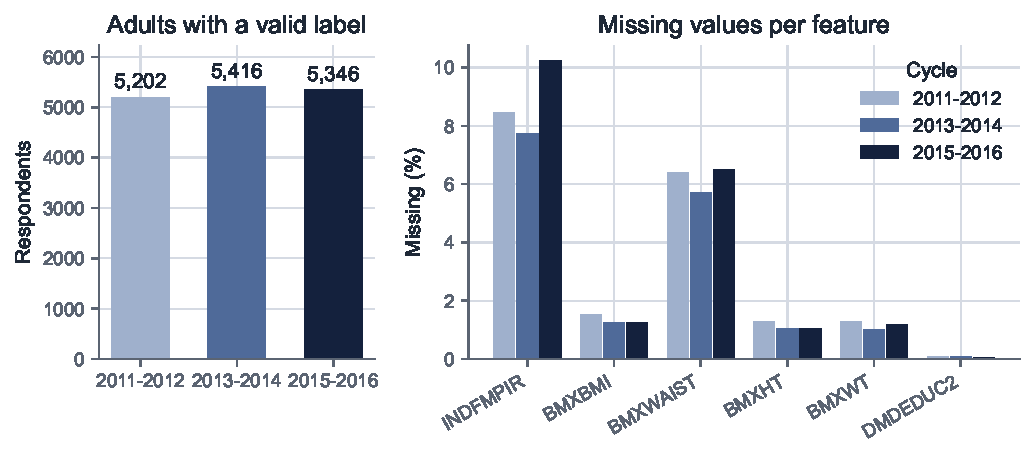
\includegraphics[width=\linewidth]{fig01_dataset_characteristics.pdf}
\caption{Respondents per cycle and missing values per feature.}
\label{fig:dataset}
\end{figure}

\begin{figure}[t]
\centering
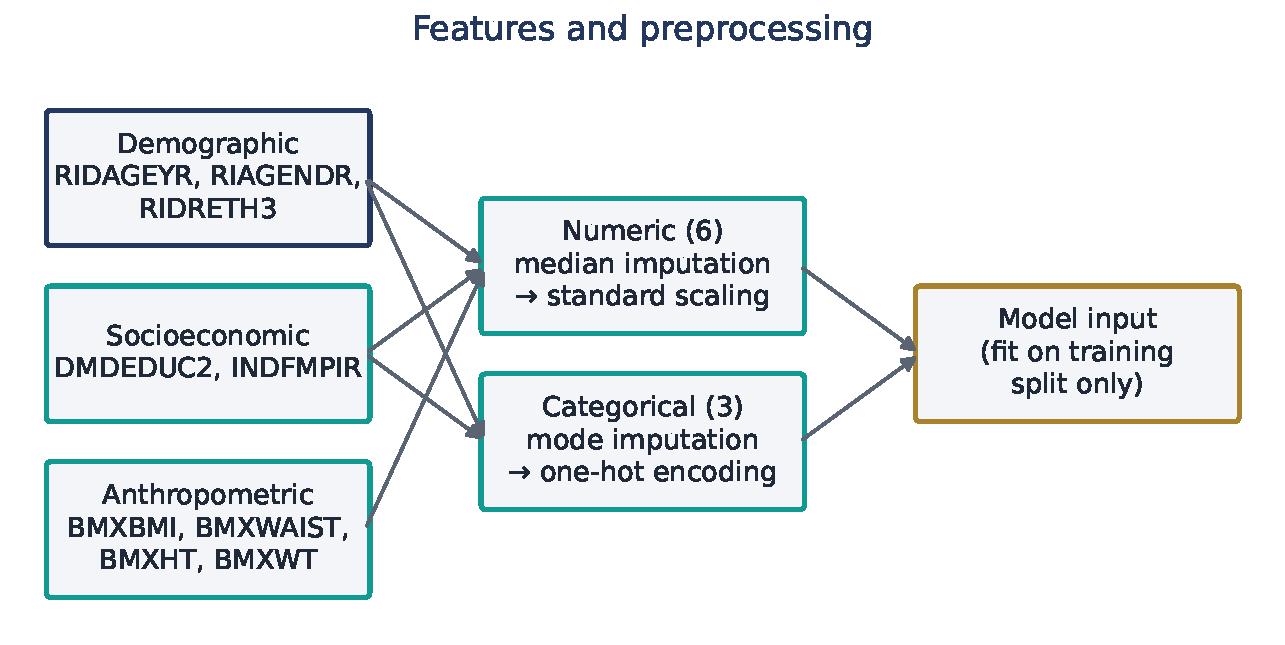
\includegraphics[width=\linewidth]{d04_features.pdf}
\caption{Feature groups and the preprocessing applied to them.}
\label{fig:features}
\end{figure}

\subsection{Evaluation protocols}
\emph{Protocol A} trains on 2011--2012, tunes on 2013--2014 and tests once on 2015--2016.
\emph{Protocol A2} splits 2011--2012 80/20 (stratified) and scores the same fitted model on the
in-period 20\% and on 2015--2016. \emph{Protocol B} pools all cycles and splits them 70/15/15
(stratified, five seeds). Five-fold stratified cross-validation is run on the development data of A
and B (Fig.~\ref{fig:methodology}).

\begin{figure*}[t]
\centering
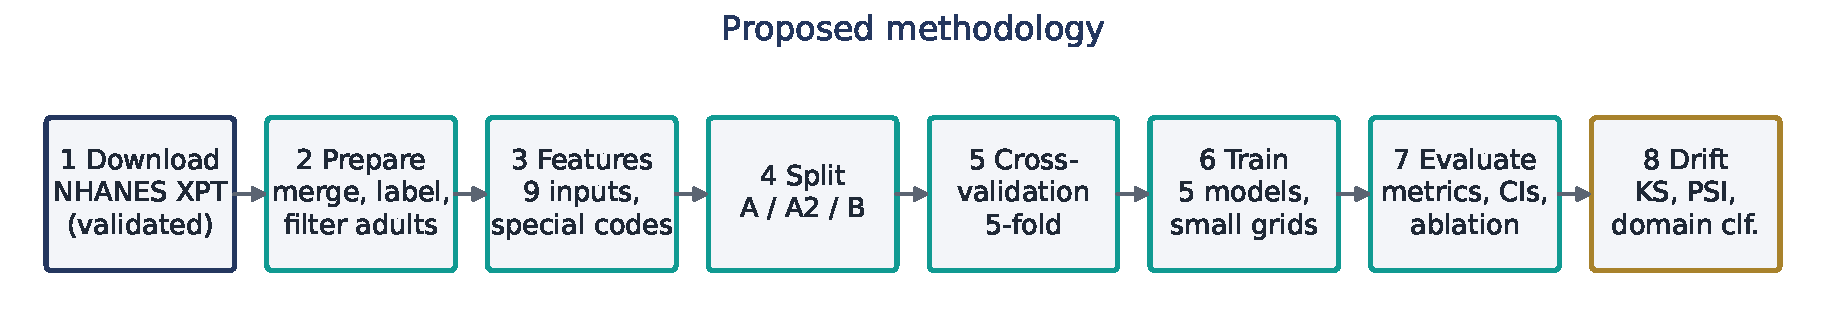
\includegraphics[width=\textwidth]{d01_methodology.pdf}
\caption{Proposed methodology (eight steps).}
\label{fig:methodology}
\end{figure*}

\subsection{Models and mathematical formulation}
Logistic regression models the probability of diabetes as
\begin{equation}
P(y=1\mid\mathbf{x}) = \sigma(\mathbf{w}^\top\mathbf{x}+b) = \frac{1}{1+e^{-(\mathbf{w}^\top\mathbf{x}+b)}}.
\end{equation}
With $TP, FP, FN, TN$ the confusion-matrix counts at threshold $\tau$,
\begin{equation}
P=\frac{TP}{TP+FP},\quad R=\frac{TP}{TP+FN},\quad F_1=\frac{2PR}{P+R}.
\end{equation}
ROC-AUC is the probability that a random positive is ranked above a random negative; PR-AUC is
computed as average precision, $\mathrm{AP}=\sum_k (R_k-R_{k-1})P_k$. The Brier score is
$\frac{1}{n}\sum_i (p_i-y_i)^2$. The threshold maximising $F_1$ on validation is
$\tau^\ast=\arg\max_\tau F_1(\tau)$. For drift we use the two-sample Kolmogorov--Smirnov statistic
\begin{equation}
D=\sup_x \lvert F_{\text{ref}}(x)-F_{\text{cmp}}(x)\rvert
\end{equation}
and the population stability index with $B$ quantile bins fixed on the reference cycle,
\begin{equation}
\mathrm{PSI}=\sum_{b=1}^{B}(q_b-p_b)\ln\frac{q_b}{p_b}.
\end{equation}
Cross-validation reports $\bar{m}=\frac{1}{K}\sum_{k=1}^K m_k$ and
$s=\sqrt{\frac{1}{K-1}\sum_k (m_k-\bar m)^2}$, and a 95\% percentile bootstrap interval uses
the 2.5th and 97.5th percentiles of the metric over $1000$ resamples:
\begin{equation}
\mathrm{CI}_{95\%}=\left[\hat\theta^\ast_{(0.025)},\ \hat\theta^\ast_{(0.975)}\right].
\end{equation}

\section{Implementation and System Design}
The pipeline is a small Python package with one command-line entry point (download, prepare, train,
drift, figures, report, presentation, notebook). All models share one scikit-learn
\texttt{ColumnTransformer} fitted on the training split only (Fig.~\ref{fig:architecture}).
Class imbalance is handled with balanced class weights (LR, RF), \texttt{scale\_pos\_weight}
(XGBoost, LightGBM) and balanced sample weights (MLP). Each model has at most six hyperparameter
configurations, selected by validation PR-AUC. The MLP is trained one epoch at a time with early
stopping on validation loss (Algorithm~\ref{alg:main}). Table~\ref{tab:stack} lists the software.

\begin{figure*}[t]
\centering
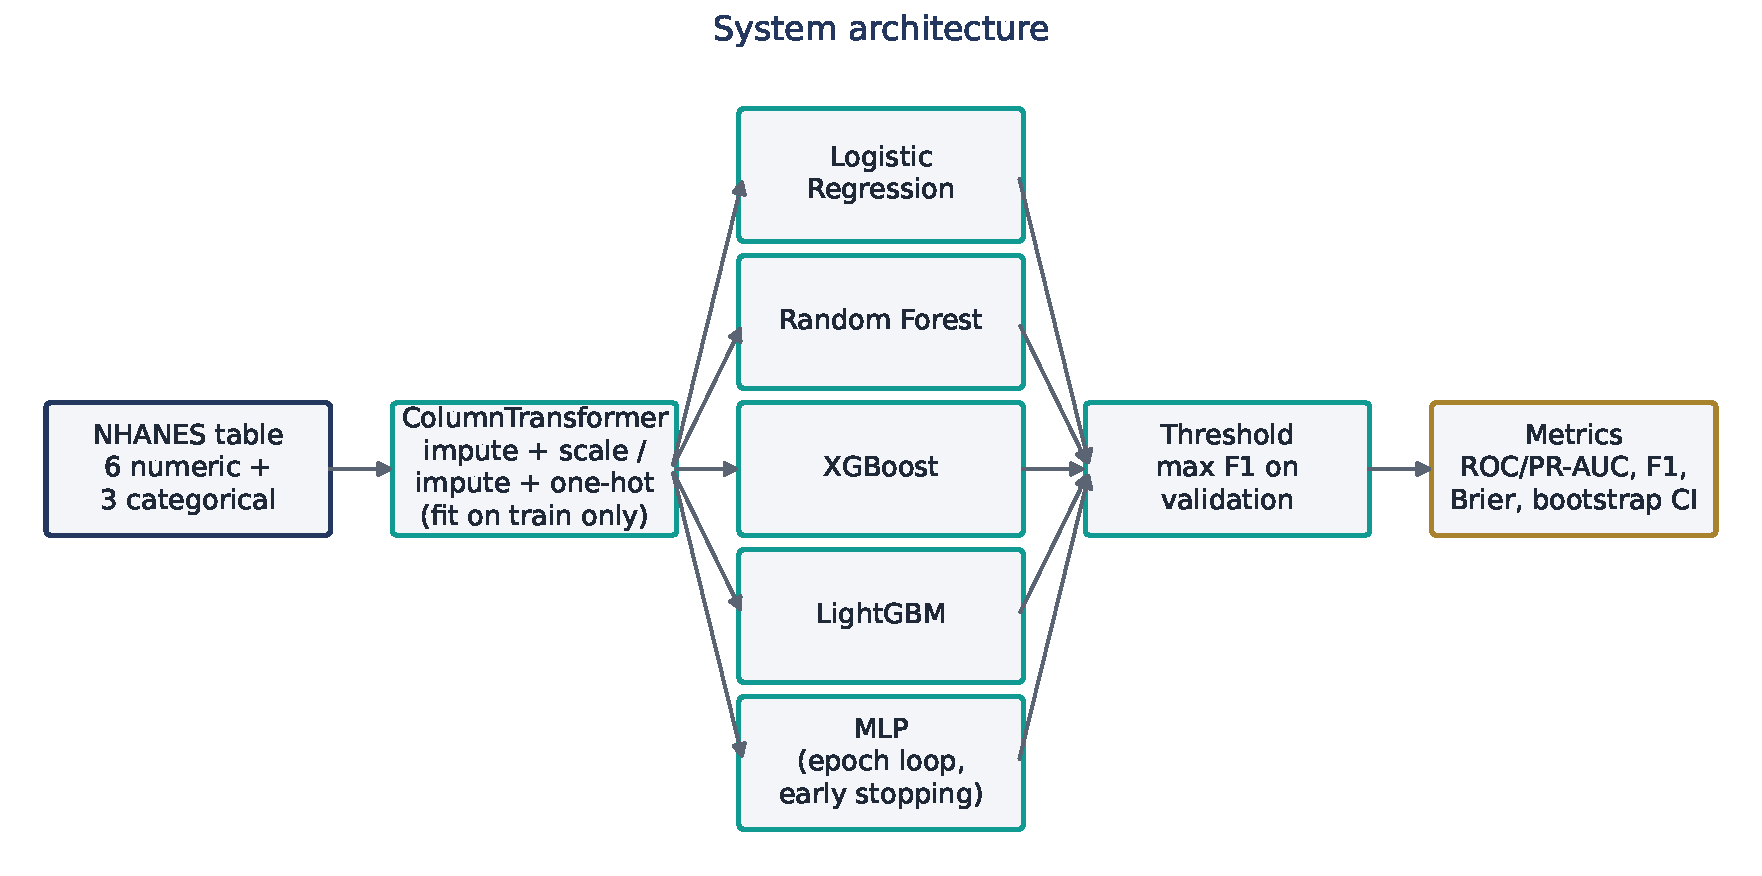
\includegraphics[width=0.9\textwidth]{d02_architecture.pdf}
\caption{System architecture: shared preprocessing, five models, threshold selection and metrics.}
\label{fig:architecture}
\end{figure*}

\begin{algorithm}[t]
\caption{Temporal benchmark for one protocol}
\label{alg:main}
\begin{algorithmic}[1]
\Require training, validation and test splits; grids $G_m$ for models $m$; seed $s$
\For{each model $m$}
  \For{each configuration $\theta \in G_m$}
    \State fit preprocessing on training split only
    \If{$m$ is MLP}
      \For{epoch $e=1,\dots,E_{\max}$}
        \State one pass of \texttt{partial\_fit}; record losses
        \State keep weights with lowest validation loss
        \State \textbf{break} if no improvement for $p$ epochs
      \EndFor
    \Else
      \State fit model $m_\theta$ on training split
    \EndIf
    \State score validation PR-AUC (ROC-AUC breaks ties)
  \EndFor
  \State $\theta^\ast \gets$ best configuration; $\tau^\ast \gets \arg\max_\tau F_1$ on validation
  \State evaluate on test at $\tau=0.5$ and $\tau^\ast$; bootstrap 95\% CIs
\EndFor
\State select best model on validation; run ablation and paired bootstrap
\end{algorithmic}
\end{algorithm}

\begin{table}[t]
\centering
\footnotesize
\caption{Technology stack (versions recorded at run time).}
\label{tab:stack}
\begin{tabular}{lrr}
\toprule
Tool & Version & Purpose \\
\midrule
Python & 3.12.13 & language \\
pandas & 3.1.1 & tables, XPT reading \\
numpy & 2.5.4 & arrays \\
scikit-learn & 1.9.1 & pipeline, LR, RF, MLP, metrics \\
xgboost & 3.4.1 & gradient boosting \\
lightgbm & 4.7.0 & gradient boosting \\
scipy & 1.18.1 & KS test \\
matplotlib & 3.11.2 & figures \\
pyyaml & 6.0.3 & configuration \\
requests & 2.34.2 & data download \\
\bottomrule
\end{tabular}
\end{table}


\section{Evaluation and Results}
Table~\ref{tab:comparison} reports all metrics on the chronological test set and
Fig.~\ref{fig:auc} shows ROC-AUC and PR-AUC with bootstrap confidence intervals.
Table~\ref{tab:protocols} and Fig.~\ref{fig:protocols} compare the three protocols, and
Table~\ref{tab:cv} gives the cross-validation folds. The MLP stopped at epoch \kn{mlp_best_epoch}
(Fig.~\ref{fig:mlp}). Figs.~\ref{fig:roc} and~\ref{fig:cm} show ROC curves and the confusion matrix
of \kn{best_model}. Table~\ref{tab:ablation} and Fig.~\ref{fig:ablation} report the ablation, and
Table~\ref{tab:drift} and Fig.~\ref{fig:drift} the drift analysis. Table~\ref{tab:literature} places
our accuracy next to published values on a different diabetes dataset.

\begin{table*}[t]
\centering
\footnotesize
\caption{Chronological test set (2015-2016), validation-tuned thresholds; 95\% bootstrap CIs.}
\label{tab:comparison}
\begin{tabular}{lrrrrrrrr}
\toprule
Model & Acc. & Prec. & Rec. & F1 & ROC-AUC [95\% CI] & PR-AUC [95\% CI] & Brier & Train (s) \\
\midrule
Logistic Regression & 0.767 & 0.343 & 0.594 & 0.435 & 0.790 [0.774, 0.805] & 0.364 [0.336, 0.399] & 0.198 & 0.01 \\
Random Forest & 0.772 & 0.350 & 0.588 & 0.438 & 0.790 [0.775, 0.807] & 0.362 [0.332, 0.396] & 0.149 & 0.30 \\
XGBoost & 0.752 & 0.336 & 0.656 & 0.444 & 0.791 [0.775, 0.807] & 0.368 [0.339, 0.402] & 0.186 & 0.09 \\
LightGBM & 0.747 & 0.331 & 0.661 & 0.441 & 0.785 [0.769, 0.800] & 0.360 [0.330, 0.394] & 0.186 & 0.11 \\
MLP & 0.744 & 0.325 & 0.646 & 0.433 & 0.792 [0.777, 0.807] & 0.362 [0.333, 0.394] & 0.193 & 0.26 \\
\bottomrule
\end{tabular}
\end{table*}

\begin{table*}[t]
\centering
\footnotesize
\caption{Test ROC-AUC under the three evaluation protocols.}
\label{tab:protocols}
\begin{tabular}{lrrrr}
\toprule
Model & A2 in-period & A2 future & A chronological & B random (mean $\pm$ std) \\
\midrule
Logistic Regression & 0.813 & 0.788 & 0.790 & 0.799 $\pm$ 0.011 \\
Random Forest & 0.821 & 0.792 & 0.790 & 0.804 $\pm$ 0.012 \\
XGBoost & 0.823 & 0.787 & 0.791 & 0.804 $\pm$ 0.015 \\
LightGBM & 0.819 & 0.783 & 0.785 & 0.803 $\pm$ 0.015 \\
MLP & 0.822 & 0.791 & 0.792 & 0.805 $\pm$ 0.011 \\
\bottomrule
\end{tabular}
\end{table*}

\begin{table*}[t]
\centering
\footnotesize
\caption{5-fold stratified cross-validation ROC-AUC on development data.}
\label{tab:cv}
\begin{tabular}{lrrrrrrr}
\toprule
Protocol & Model & Fold 1 & Fold 2 & Fold 3 & Fold 4 & Fold 5 & Mean $\pm$ std \\
\midrule
B & LightGBM & 0.801 & 0.816 & 0.812 & 0.800 & 0.797 & 0.805 $\pm$ 0.008 \\
B & Logistic Regression & 0.796 & 0.812 & 0.806 & 0.806 & 0.794 & 0.803 $\pm$ 0.007 \\
B & MLP & 0.804 & 0.819 & 0.809 & 0.808 & 0.800 & 0.808 $\pm$ 0.007 \\
B & Random Forest & 0.795 & 0.818 & 0.805 & 0.799 & 0.795 & 0.802 $\pm$ 0.009 \\
B & XGBoost & 0.805 & 0.817 & 0.813 & 0.805 & 0.797 & 0.807 $\pm$ 0.008 \\
A & LightGBM & 0.805 & 0.796 & 0.809 & 0.814 & 0.798 & 0.804 $\pm$ 0.008 \\
A & Logistic Regression & 0.813 & 0.799 & 0.800 & 0.807 & 0.794 & 0.803 $\pm$ 0.008 \\
A & MLP & 0.809 & 0.790 & 0.809 & 0.806 & 0.799 & 0.803 $\pm$ 0.008 \\
A & Random Forest & 0.797 & 0.787 & 0.807 & 0.805 & 0.791 & 0.798 $\pm$ 0.009 \\
A & XGBoost & 0.806 & 0.798 & 0.813 & 0.809 & 0.796 & 0.804 $\pm$ 0.007 \\
\bottomrule
\end{tabular}
\end{table*}

\begin{table*}[t]
\centering
\footnotesize
\caption{Ablation of the validation-selected model on the 2015-2016 test set.}
\label{tab:ablation}
\begin{tabular}{lrrrrrr}
\toprule
Configuration & ROC-AUC & PR-AUC & F1 & $\Delta$ROC-AUC & $\Delta$PR-AUC & $\Delta$F1 \\
\midrule
full model & 0.791 & 0.368 & 0.444 & +0.000 & +0.000 & +0.000 \\
without demographic features & 0.705 & 0.265 & 0.356 & -0.086 & -0.103 & -0.088 \\
without socioeconomic features & 0.792 & 0.369 & 0.441 & +0.000 & +0.001 & -0.003 \\
without anthropometric features & 0.748 & 0.297 & 0.396 & -0.043 & -0.071 & -0.048 \\
no class-imbalance handling & 0.789 & 0.364 & 0.440 & -0.002 & -0.005 & -0.005 \\
threshold 0.5 instead of tuned & 0.791 & 0.368 & 0.429 & +0.000 & +0.000 & -0.015 \\
\bottomrule
\end{tabular}
\end{table*}

\begin{table}[t]
\centering
\footnotesize
\caption{Numeric feature drift, 2015-2016 vs 2011-2012.}
\label{tab:drift}
\begin{tabular}{lrrrrr}
\toprule
Feature & Mean 2011-12 & Mean 2015-16 & KS & PSI & Missing 2015-16 \\
\midrule
RIDAGEYR & 48.54 & 49.20 & 0.022 & 0.010 & 0.0\% \\
INDFMPIR & 2.42 & 2.43 & 0.056 & 0.029 & 10.3\% \\
BMXBMI & 28.71 & 29.50 & 0.057 & 0.018 & 1.3\% \\
BMXWAIST & 98.15 & 100.10 & 0.056 & 0.016 & 6.5\% \\
BMXHT & 167.25 & 166.11 & 0.051 & 0.016 & 1.0\% \\
BMXWT & 80.53 & 81.65 & 0.024 & 0.005 & 1.2\% \\
\bottomrule
\end{tabular}
\end{table}

\begin{table*}[t]
\centering
\footnotesize
\caption{Accuracy reported by TableShift for its BRFSS Diabetes task next to ours. Datasets, shifts and thresholds differ, so the values are not directly comparable.}
\label{tab:literature}
\begin{tabular}{llllr}
\toprule
Method & Source & Dataset & Test set & Accuracy \\
\midrule
XGBoost & \cite{gardner2023tableshift} & BRFSS Diabetes (TableShift) & In-distribution test (White non-Hispanic) & 0.877 \\
XGBoost & \cite{gardner2023tableshift} & BRFSS Diabetes (TableShift) & Out-of-distribution test (other race/ethnicity groups) & 0.832 \\
LightGBM & \cite{gardner2023tableshift} & BRFSS Diabetes (TableShift) & In-distribution test (White non-Hispanic) & 0.876 \\
LightGBM & \cite{gardner2023tableshift} & BRFSS Diabetes (TableShift) & Out-of-distribution test (other race/ethnicity groups) & 0.833 \\
MLP & \cite{gardner2023tableshift} & BRFSS Diabetes (TableShift) & In-distribution test (White non-Hispanic) & 0.877 \\
MLP & \cite{gardner2023tableshift} & BRFSS Diabetes (TableShift) & Out-of-distribution test (other race/ethnicity groups) & 0.832 \\
XGBoost & This work & NHANES adults (DIQ010) & A2 in-period holdout (2011-2012) & 0.813 \\
XGBoost & This work & NHANES adults (DIQ010) & A2 future cycle (2015-2016) & 0.785 \\
LightGBM & This work & NHANES adults (DIQ010) & A2 in-period holdout (2011-2012) & 0.809 \\
LightGBM & This work & NHANES adults (DIQ010) & A2 future cycle (2015-2016) & 0.779 \\
MLP & This work & NHANES adults (DIQ010) & A2 in-period holdout (2011-2012) & 0.764 \\
MLP & This work & NHANES adults (DIQ010) & A2 future cycle (2015-2016) & 0.743 \\
\bottomrule
\end{tabular}
\end{table*}


\begin{figure}[t]
\centering
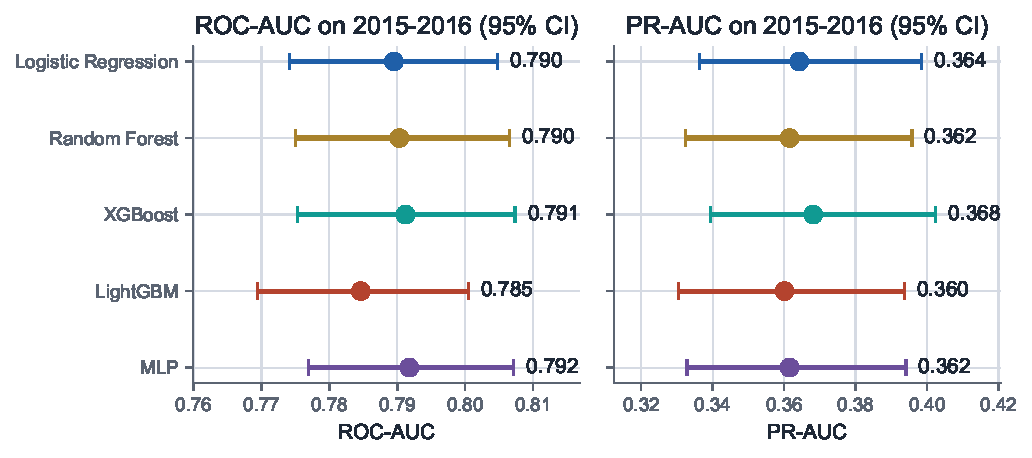
\includegraphics[width=\linewidth]{fig03_auc_ci.pdf}
\caption{Chronological-test ROC-AUC and PR-AUC with 95\% bootstrap CIs.}
\label{fig:auc}
\end{figure}

\begin{figure}[t]
\centering
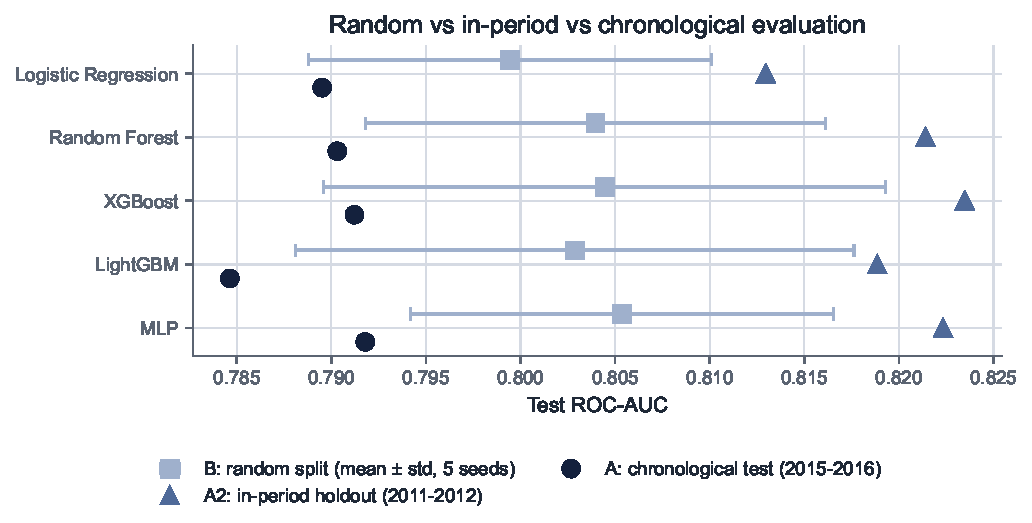
\includegraphics[width=\linewidth]{fig04_random_vs_temporal.pdf}
\caption{Test ROC-AUC under random, in-period and chronological evaluation.}
\label{fig:protocols}
\end{figure}

\begin{figure}[t]
\centering
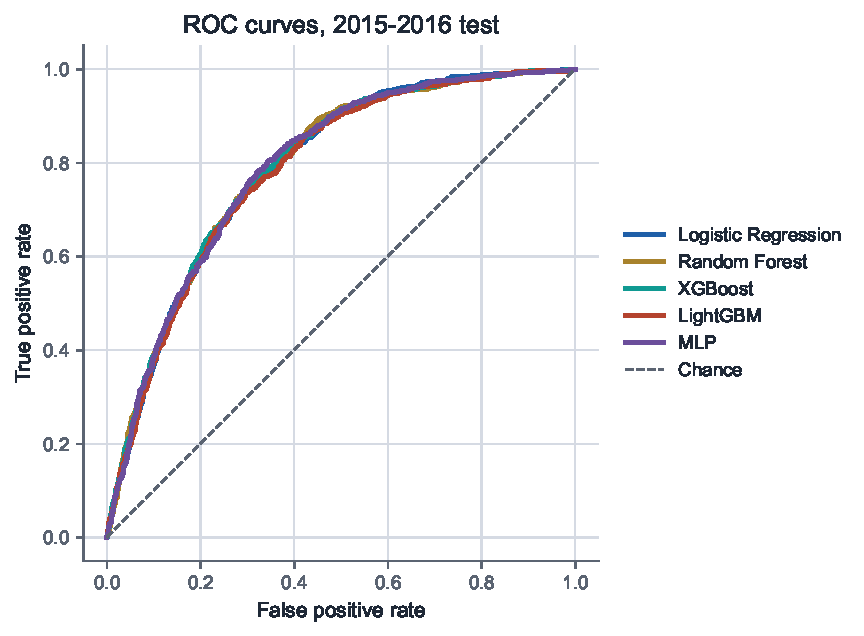
\includegraphics[width=0.85\linewidth]{fig05_roc_curves.pdf}
\caption{ROC curves on the 2015--2016 test set.}
\label{fig:roc}
\end{figure}

\begin{figure}[t]
\centering
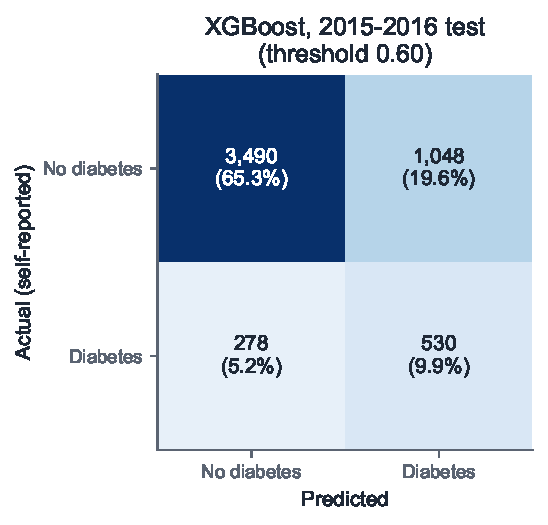
\includegraphics[width=0.6\linewidth]{fig06_confusion_matrix.pdf}
\caption{Confusion matrix of the validation-selected model on 2015--2016.}
\label{fig:cm}
\end{figure}

\begin{figure}[t]
\centering
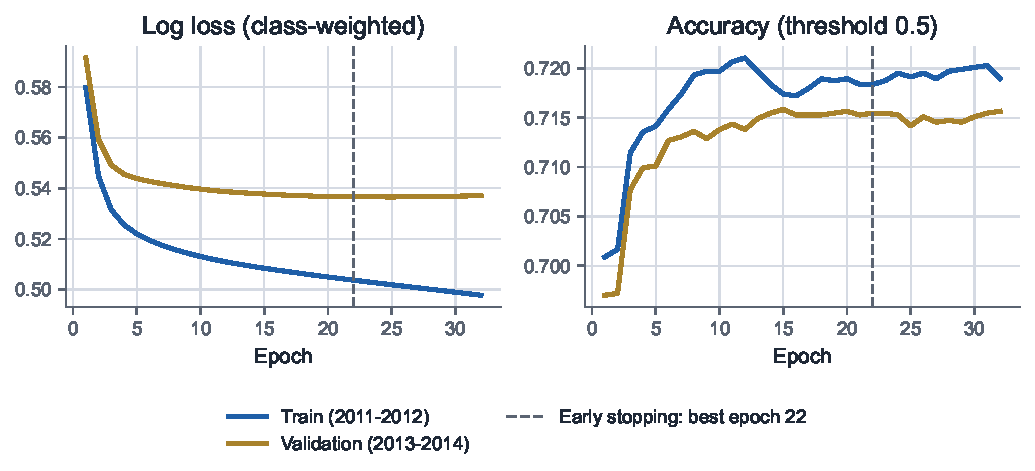
\includegraphics[width=\linewidth]{fig08_mlp_curves.pdf}
\caption{MLP training and validation curves with the early-stopping epoch.}
\label{fig:mlp}
\end{figure}

\begin{figure}[t]
\centering
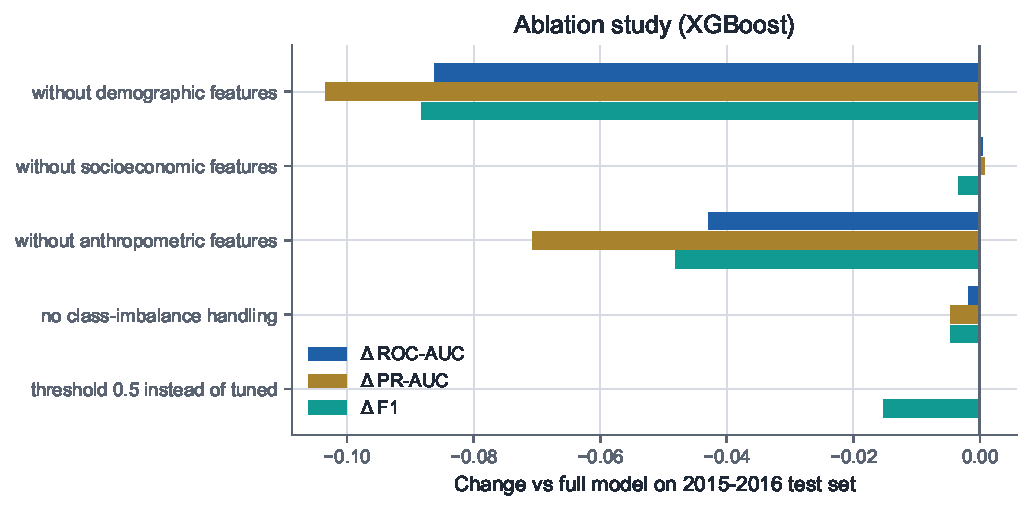
\includegraphics[width=\linewidth]{fig09_ablation.pdf}
\caption{Ablation: change in test metrics when one component is removed.}
\label{fig:ablation}
\end{figure}

\begin{figure}[t]
\centering
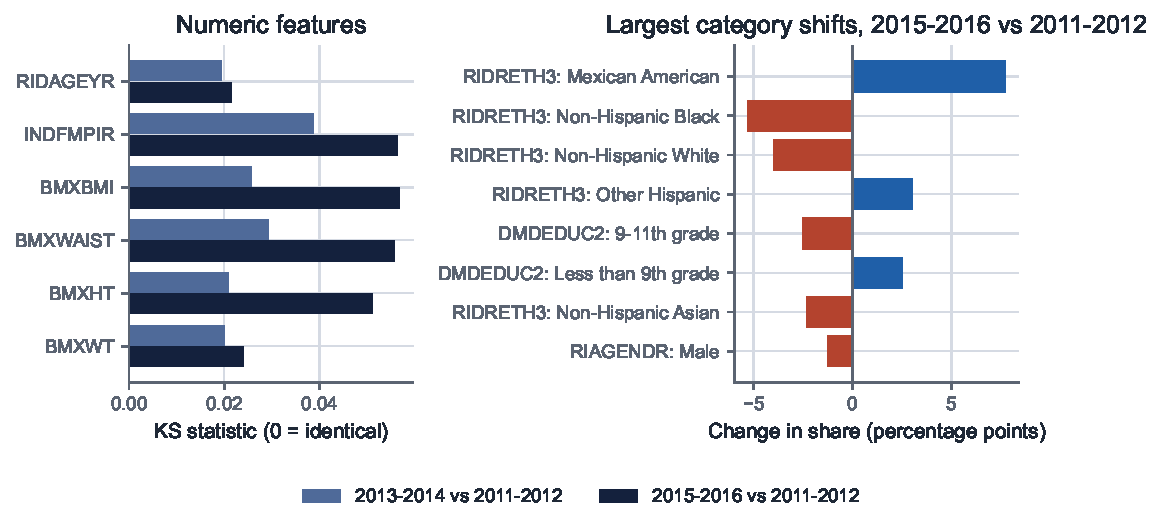
\includegraphics[width=\linewidth]{fig07_feature_drift_ks.pdf}
\caption{Feature drift relative to 2011--2012.}
\label{fig:drift}
\end{figure}

\begin{figure}[t]
\centering
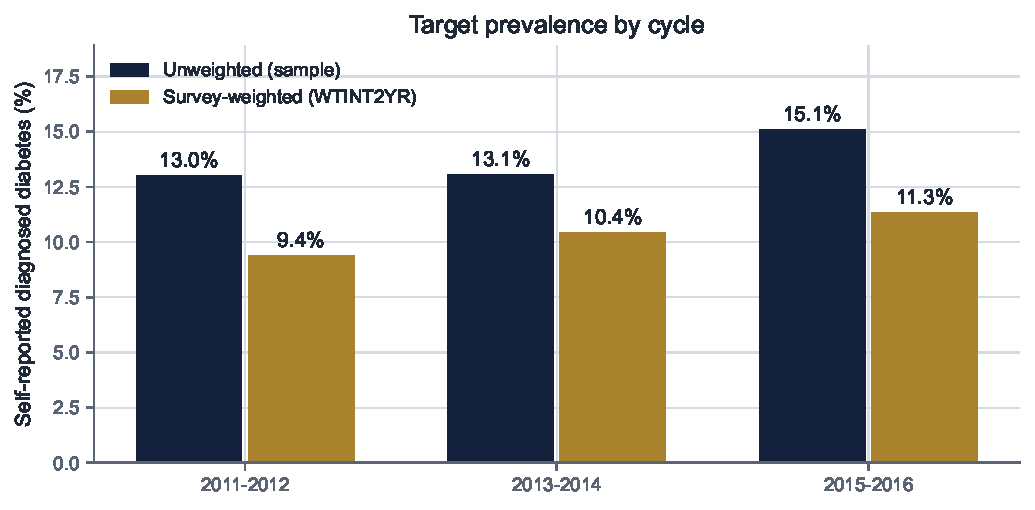
\includegraphics[width=\linewidth]{fig02_prevalence.pdf}
\caption{Unweighted and survey-weighted prevalence by cycle.}
\label{fig:prevalence}
\end{figure}

\section{Discussion}
\STUDENT{Interpret the results for RQ1--RQ4 using only the numbers in the tables and figures.
Points to address: whether model differences are conclusive given the paired bootstrap; what the
random-vs-chronological gap and the A2 gap (with their CIs) say about temporal degradation; how the
rise in prevalence (Fig.~\ref{fig:prevalence}) affects PR-AUC and thresholds; and what the ablation
shows about feature groups.}

\textbf{Limitations and threats to validity.} NHANES is a cross-sectional population survey, not
longitudinal hospital EHR data, so each cycle contains different people. Models are trained
unweighted, so results describe the sample rather than the US population. The label is
self-reported diagnosed diabetes, so undiagnosed diabetes counts as negative. Body measurements are
taken after a possible diagnosis, so associations may partly reflect reverse causation. Random and
chronological test sets contain different respondents, so their difference is not purely a time
effect. We describe observed distribution changes and do not attribute them to causes such as
sampling design or diagnosis practice without external evidence.

\section{Conclusion and Future Work}
\STUDENT{Summarise the main finding in two or three sentences and propose concrete future work
(e.g., more cycles, survey-weighted training, calibration under shift, laboratory-free risk scores).}

\bibliographystyle{IEEEtran}
\bibliography{references}

\end{document}
